\section{Safety}
\label{membership:safety}

Preserving safety is the first challenge for configuration changes.
For the mechanism to be safe,
there must be no point during the transition where it is possible for
two leaders to be elected for the same term. If a single configuration
change adds or removes many servers, switching the cluster directly from
the old configuration to the new configuration can be unsafe;
it isn't possible to atomically switch all of the servers at once, so 
the cluster can potentially split into two independent majorities
during the transition (see
Figure~\ref{fig:membership:reconfigurationdifficulty}).

\begin{figure}
\centering
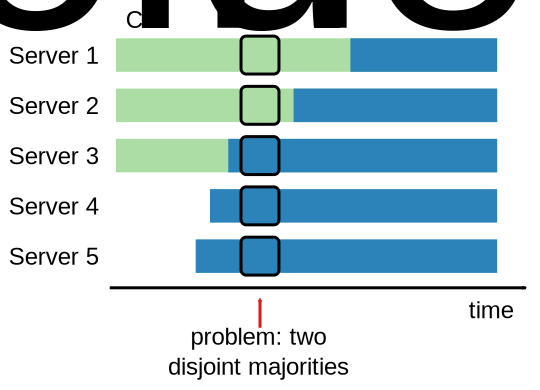
\includegraphics[scale=.50]{membership/reconfigurationdifficulty}
\vcaption[safety challenge]{
Switching directly from one configuration to another can be
unsafe because different servers will switch at different times.
In this example, the cluster grows from three servers to five.
Unfortunately, there is a point in time where two different leaders
can be elected for the same term,
one with a majority of the old
configuration (\cold{}) and another with a majority of the new
configuration (\cnew{}).
}
\label{fig:membership:reconfigurationdifficulty}
\end{figure}

\begin{figure}
\centering

\begin{subfigure}{.45\textwidth}
\centering
\includegraphics[scale=0.50]{membership/special4to5}
\caption{
Adding one server to a 4-server cluster.
}
\end{subfigure}
~
\begin{subfigure}{.45\textwidth}
\centering
\includegraphics[scale=0.50]{membership/special3to4}
\caption{
Adding one server to a 3-server cluster.
}
\end{subfigure}

\vspace{3ex}

\begin{subfigure}{.45\textwidth}
\centering
\includegraphics[scale=0.50]{membership/special5to4}
\caption{
Removing one server from a 5-server cluster.
}
\end{subfigure}
~
\begin{subfigure}{.45\textwidth}
\centering
\includegraphics[scale=0.50]{membership/special4to3}
\caption{
Removing one server from a 4-server cluster.
}
\end{subfigure}

\vcaption[adding/removing one server maintains overlap]{
The addition and removal of a single server from an even- and an
odd-sized cluster.
In each figure,
the blue rectangle shows a majority of the old cluster, and the red
rectangle shows a majority of the new cluster.
In every single-server membership change, an overlap between any majority
of the old cluster and any majority of the new cluster is preserved,
as needed for safety. For example in (b), a majority of the old cluster
must include two of the left three servers, and a majority of the new
cluster must include three of the servers in the new cluster, of which
at least two must come from the old cluster.
}
\label{fig:membership:special}
\end{figure}

Most membership change algorithms introduce additional mechanism to deal
with such problems. This is what we did for Raft initially, but we later
discovered a simpler approach, which is to disallow membership changes
that could result in disjoint majorities. Thus, Raft restricts the types
of changes that are allowed: only one server can be added or removed
from the cluster at a time. More complex changes in membership are
implemented as a series of single-server changes. Most of this chapter
describes the single-server approach, which is easier to understand than
our original approach. For completeness,
Section~\ref{membership:arbitrary} describes the original approach,
which incurs additional complexity to handle arbitrary configuration
changes. We implemented the more complex approach in LogCabin prior to
discovering the simpler single-server change approach; it still uses the
more complex approach at the time of this writing.

When adding a single server to a cluster or removing a single server
from a cluster, any majority of the old cluster overlaps with any
majority of the new cluster; see Figure~\ref{fig:membership:special}.
This overlap prevents the cluster from splitting into two independent
majorities; in terms of the safety argument of
Section~\ref{basicraft:safety:argument}, it guarantees the existence of
``the voter''. Thus, when adding or removing just a single server, it is
safe to switch directly to the new configuration. Raft exploits this
property to change cluster membership safely using little additional
mechanism.

Cluster configurations are stored and communicated using special entries
in the replicated log.
This leverages the existing mechanisms in Raft to
replicate and persist configuration information.
It also allows the cluster to continue to service
client requests while configuration changes are in progress,
by imposing ordering between
configuration changes and client requests (while allowing both to be
replicated concurrently in a pipeline and/or in batches).

When the leader receives a request to add or remove a server from its
current configuration (\cold{}), it appends the new configuration
(\cnew{}) as an entry in its log and replicates that entry using the
normal Raft mechanism. The new configuration takes effect on each server
as soon as it is added to that server's log: the \cnew{} entry is
replicated to the \cnew{} servers, and a majority of the new
configuration is used to determine the \cnew{} entry's commitment. This
means that servers do not wait for configuration entries to be
committed, and each server always uses the latest configuration found in
its log.

The configuration change is complete once the \cnew{} entry is
committed. At this point, the leader knows that a majority of the
\cnew{} servers have adopted \cnew{}. It also knows that any servers
that have not moved to \cnew{} can no longer form a majority of the
cluster, and servers without \cnew{} cannot be elected leader.
Commitment of \cnew{} allows three things to continue:
%
\begin{enumerate}
%
\item The leader can acknowledge the successful completion of the
configuration change.
%
\item If the configuration change removed a server, that server can be
shut down.
%
\item Further configuration changes can be started. Before this point,
overlapped configuration changes could degrade to unsafe situations
like the one in Figure~\ref{fig:membership:reconfigurationdifficulty}.
%
\end{enumerate}

As stated above, servers always use the latest configuration in their
logs, regardless of whether that configuration entry has been committed.
This allows leaders to easily avoid overlapping configuration changes
(the third item above), by not beginning a new change until the previous
change's entry has committed. It is only safe to start another membership
change once a majority of the old cluster has moved to operating under
the rules of \cnew{}. If servers adopted \cnew{} only when they
learned that \cnew{} was committed, Raft leaders would have a difficult
time knowing when a majority of the old cluster had adopted it. They
would need to track which servers know of the entry's commitment, and
the servers would need to persist their commit index to disk; neither of
these mechanisms is required in Raft. Instead, each server
adopts \cnew{} as soon as that entry exists in its log, and the leader
knows it's safe to allow further configuration changes as soon as the
\cnew{} entry has been committed. Unfortunately, this decision does
imply that a log entry for a configuration change can be removed (if
leadership changes); in this case, a server must be prepared to fall
back to the previous configuration in its log.

In Raft, it is the caller's configuration that is used in reaching
consensus, both for voting and for log replication:
%
\begin{itemize}
%
\item A server accepts AppendEntries requests from a leader that
is not part of the server's latest configuration. Otherwise, a new server
could never be added to the cluster (it would never accept any log entries
preceding the configuration entry that adds the server).
%
\item A server also grants its vote to a candidate that is not
part of the server's latest configuration (if the candidate has a
sufficiently up-to-date log and a current term). This vote may
occasionally be needed to keep the cluster available. For example,
consider adding a fourth server to a three-server cluster. If one server
were to fail, the new server's vote would be needed to form a majority
and elect a leader.
%
\end{itemize}
%
Thus, servers process incoming RPC requests without consulting their
current configurations.

